%%%%%%%%%%%%%%%%%%%%%%%%%%%%%%%%%%%%%%%%%%%%%%%%%%%%%%%%%%%%%%%%%%%%%%%%%%
%
% StMcEvent - User Guide and Reference Manual -- LaTeX Source
%
% $Id: StMcEvent.tex,v 1.1.1.1 1999/07/13 18:28:19 uid2620 Exp $
%
% Authors:Michael A. Lisa
%         Thomas S. Ullrich
%         Manuel Calderon de la Barca Sanchez
%
%%%%%%%%%%%%%%%%%%%%%%%%%%%%%%%%%%%%%%%%%%%%%%%%%%%%%%%%%%%%%%%%%%%%%%%%%%
%
% Notes to the authors:
%
% - A template for a class reference is at the end of this file.
% - Wrap all names functions with \name{}
% - All code, examples, prototypes in \verb+ ... +\\
%   or \begin{verbatim} ... \end{verbatim}
% - Use \StMcEvent if you refer to the package itself (not the class)
%
% This file is best edit with xemacs and the 'Function' package loaded.
%
%%%%%%%%%%%%%%%%%%%%%%%%%%%%%%%%%%%%%%%%%%%%%%%%%%%%%%%%%%%%%%%%%%%%%%%%%%
%
% $Log: StMcEvent.tex,v $
% Revision 1.1.1.1  1999/07/13 18:28:19  uid2620
% Initial import
%
%
%%%%%%%%%%%%%%%%%%%%%%%%%%%%%%%%%%%%%%%%%%%%%%%%%%%%%%%%%%%%%%%%%%%%%%%%%%
\documentclass[twoside]{article}

\parindent 0pt
\parskip 6pt
\advance\textwidth by 80pt%
\advance\evensidemargin by -80pt%

\usepackage{graphicx}
\usepackage{psboxit}
\usepackage{amsmath}
\usepackage{amssymb}
\usepackage{amsfonts}
\usepackage{fancyhdr}
\usepackage{times}
\usepackage{verbatim}
\usepackage{makeidx}

\PScommands      % init boxit
\makeindex

%%%%%%%%%%%%%%%%%%%%%%%%%%%%%%%%%%%%%%%%%%%%%%%%%%%%%%%%%%%%%%%%%%%%
%
% Define header and footer style
%
%%%%%%%%%%%%%%%%%%%%%%%%%%%%%%%%%%%%%%%%%%%%%%%%%%%%%%%%%%%%%%%%%%%%
\pagestyle{fancyplain}
\rhead[\fancyplain{}{\bfseries\leftmark}]
      {\fancyplain{}{\bfseries\rightmark}}
\lhead[\fancyplain{}{\bfseries\rightmark}]
      {\fancyplain{}{\bfseries\leftmark}}
\rfoot[{}]{\fancyplain{}{\bfseries\thepage}}
\lfoot[\fancyplain{}{\bfseries\thepage}]{}
\cfoot{}

%%%%%%%%%%%%%%%%%%%%%%%%%%%%%%%%%%%%%%%%%%%%%%%%%%%%%%%%%%%%%%%%%%%%
%
% Typographic Conventions
%
%%%%%%%%%%%%%%%%%%%%%%%%%%%%%%%%%%%%%%%%%%%%%%%%%%%%%%%%%%%%%%%%%%%%
\newcommand{\name}[1]{\textsl{#1}}%  class-, function-, package names
\newcommand{\StEvent}{\textsf{StEvent}}
\newcommand{\StMcEvent}{\textsf{StMcEvent}}
\newcommand{\StAssociationMaker}{\textsf{StAssociationMaker}}

%%%%%%%%%%%%%%%%%%%%%%%%%%%%%%%%%%%%%%%%%%%%%%%%%%%%%%%%%%%%%%%%%%%%
%
% Define multiline labels for class reference
%
%%%%%%%%%%%%%%%%%%%%%%%%%%%%%%%%%%%%%%%%%%%%%%%%%%%%%%%%%%%%%%%%%%%%
\newcommand{\entrylabel}[1]{\mbox{\textbf{{#1}}}\hfil}%
\newenvironment{entry}
{\begin{list}{}%
    {\renewcommand{\makelabel}{\entrylabel}%
     \setlength{\labelwidth}{90pt}%
     \setlength{\leftmargin}{\labelwidth}
     \advance\leftmargin by \labelsep%
    }%
}%
{\end{list}}

\newcommand{\Entrylabel}[1]%
{\raisebox{0pt}[1ex][0pt]{\makebox[\labelwidth][l]%
    {\parbox[t]{\labelwidth}{\hspace{0pt}\textbf{{#1}}}}}}
\newenvironment{Entry}%
{\renewcommand{\entrylabel}{\Entrylabel}\begin{entry}}%
  {\end{entry}}

\begin{document}

%%%%%%%%%%%%%%%%%%%%%%%%%%%%%%%%%%%%%%%%%%%%%%%%%%%%%%%%%%%%%%%%%%%%
%
%    Title page
%
%%%%%%%%%%%%%%%%%%%%%%%%%%%%%%%%%%%%%%%%%%%%%%%%%%%%%%%%%%%%%%%%%%%%
\begin{titlepage}
\pagestyle{empty}
\vspace*{-35mm}
\begin{center}
  \mbox{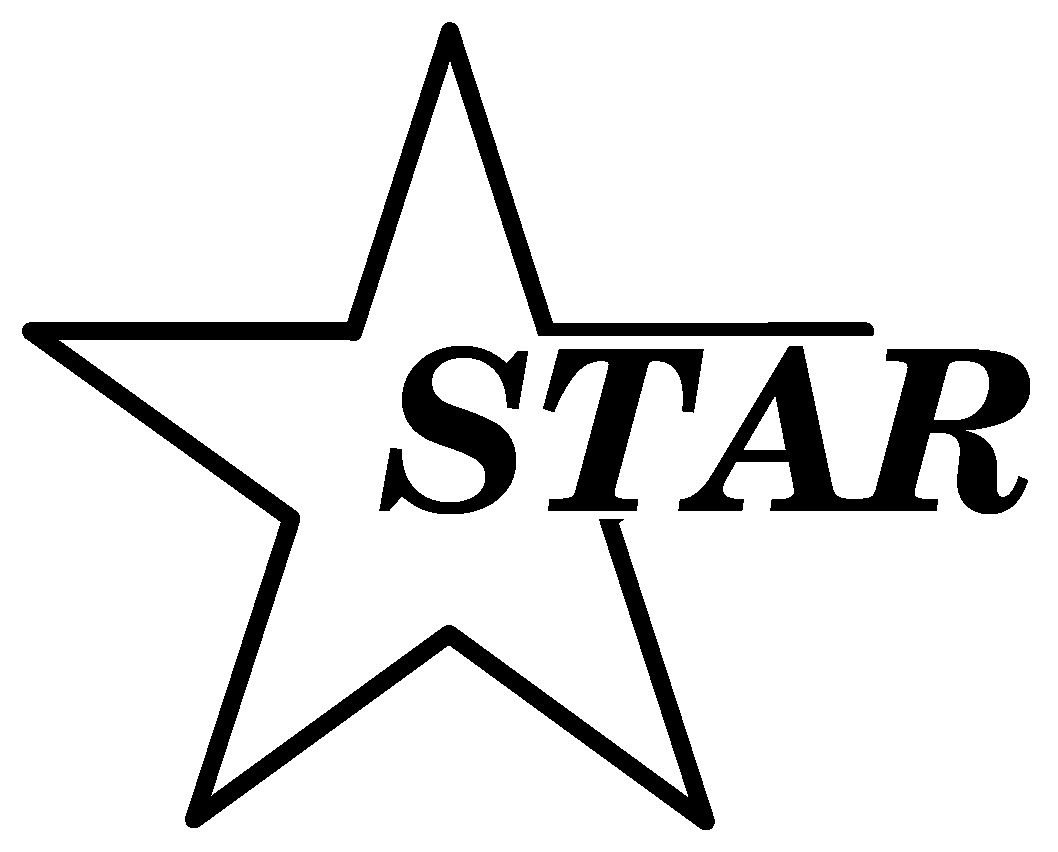
\includegraphics[width=2cm]{StarIcon.eps}}
  {\Large\bf STAR Offline Library Long Writeup}
  \hfill\mbox{}\\[3cm]
  \mbox{\includegraphics[width=\textwidth]{StMcEventTitle.eps}}
  \hfill\mbox{}\\[3cm]
  {\LARGE User Guide and Reference Manual}\\[2cm]
  {\LARGE $  $}  \\[5mm] % replaced by cvs with current revision
  {\LARGE $  $}  % replaced by cvs with current revision
  \vfill
\end{center}
\cleardoublepage
\end{titlepage}
\pagenumbering{roman}

%%%%%%%%%%%%%%%%%%%%%%%%%%%%%%%%%%%%%%%%%%%%%%%%%%%%%%%%%%%%%%%%%%%%
%
%    Table of contents
%
%%%%%%%%%%%%%%%%%%%%%%%%%%%%%%%%%%%%%%%%%%%%%%%%%%%%%%%%%%%%%%%%%%%%
\tableofcontents
\cleardoublepage

%%%%%%%%%%%%%%%%%%%%%%%%%%%%%%%%%%%%%%%%%%%%%%%%%%%%%%%%%%%%%%%%%%%%
%
%    User Guide
%
%%%%%%%%%%%%%%%%%%%%%%%%%%%%%%%%%%%%%%%%%%%%%%%%%%%%%%%%%%%%%%%%%%%%
\pagenumbering{arabic}
\part{User Guide}
\clearpage

%%%%%%%%%%%%%%%%%%%%%%%%%%%%%%%%%%%%%%%%%%%%%%%%%%%%%%%%%%%%%%%%%%%%

\section{Introduction}

\StMcEvent\footnote{We will adopt the convention used in \StEvent\ 
    and write \StMcEvent\ when we refer to the package and
    \name{StMcEvent} when we refer to the class.} is a package that
compliments the use of \StEvent\ . The aim is for the user to be able
to access and analyze Monte Carlo with the same object oriented
approach as \StEvent\ . The top class is \name{StMcEvent}, and a
pointer to this  class enables access to all the relevant Monte Carlo
information.  Again, the pointer is obtained through a Maker, in this
case \name{StMcEventMaker}.  An example invocation is found in sec.~\ref{sec:howto}.

The information contained in \StMcEvent\ is designed to be simply
a reflection of the information already available in the existing
g2t tables.  The primary keys and foreign keys are replaced by
associations between classes through pointers, like in \StEvent\ .
At the moment, not all the information found on the g2t tables is
encapsulated in \StMcEvent\ , for a full description of what is
avaliable, please refer to sec.~\ref{sec:refman}.  Also note that
\StMcEvent\ is a work in progress, and if additional information
is needed, it can be added.

The goal of \StMcEvent\ is to be used in conjunction with \StEvent\ in
order to have an OO model for both pure Monte Carlo data and DST data
that has passed through the whole reconstruction chain.  To be able
to relate the 2 packages, there is an additional package that is
run after both \StEvent\ and \StMcEvent\ are filled: \StAssociationMaker\ .
\index{StAssociationMaker}
The aim of \StAssociationMaker\ is to establish the relationships
between the reconstructed and Monte Carlo information, so that
users can easily check whether a particular reconstructed hit or
track is found, and if so to directly obtain the associated Monte
Carlo hit or track so that an assessment of the quality of the
data can be made.

\clearpage

%%%%%%%%%%%%%%%%%%%%%%%%%%%%%%%%%%%%%%%%%%%%%%%%%%%%%%%%%%%%%%%%%%%%

\section{How to read this document}

This document is divided in two parts, a user guide and a
reference manual. In the first part we rather concentrate on basic
questions and provide guidance to get started.  Some of the information
given here overlaps that one found in the \StEvent\ documentation,
and we provide it again here for completeness (We think that it is better
to be redundant than to have to remember which information is in which
manual).  The reference section
provides information on all available classes, their member functions
and related operators. The class references contain one or more
examples which demonstrate some features of each class and how to use
them.

New users should \textbf{not} start with the Reference section. It is
meant as a lookup when specific information is needed. Beginners
should study the User Guide and should make themselves familiar only
with those classes they will encounter more frequently:
\name{StMcEvent}  (sec.~\ref{sec:StMcEvent}),
\name{StMcTrack}  (sec.~\ref{sec:StMcTrack}),
\name{StMcVertex} (sec.~\ref{sec:StMcVertex}),
and \name{StMcTpcHit} (sec.~\ref{sec:StMcTpcHit}).



Understanding the various
examples certainly is the best way to get started. However, the examples
are given for illustration purposes only, and are not complete programs.

%%%%%%%%%%%%%%%%%%%%%%%%%%%%%%%%%%%%%%%%%%%%%%%%%%%%%%%%%%%%%%%%%%%%

\section{Further documentation}
\label{sec:furtherdoc}

\StMcEvent\ makes use of various classes from the StarClassLibrary (SCL).
To obtain the SCL documentation perform the following steps:
\begin{enumerate}
  \item Obtain an \name{afs} token: \name{klog -cell rhic}.
  \item Make sure \name{\$CVSROOT} is set properly: \\ %%$
	(i.e.~\name{CVSROOT = /afs/rhic/star/packages/repository})
  \item Check-out the SCL into your current working directory:\\
    \name{cvs checkout StRoot/StarClassLibrary}
  \item Go to the directory containing the documentation:\\
    \name{cd StRoot/StarClassLibrary/doc/tex}
  \item Create the PostScript document \name{StarClassLibrary.ps}:\\
    \name{make}
\end{enumerate}
\index{SCL} \index{StarClassLibrary}

%%%%%%%%%%%%%%%%%%%%%%%%%%%%%%%%%%%%%%%%%%%%%%%%%%%%%%%%%%%%%%%%%%%%

\section{Getting \StMcEvent\ Sources}  \index{Getting StMcEvent sources}

To access the complete source code proceed as follows:

\StMcEvent\ is under {\bf CVS} control at BNL.  It can
be accessed via \name{afs}: \index{afs} \index{CVS} \index{CVSROOT}
\begin{enumerate}
  \item Obtain an \name{afs} token: \name{klog -cell rhic}.
  \item Make sure \name{\$CVSROOT} is set properly:\\ %%$
    (i.e.~\name{CVSROOT = /afs/rhic/star/packages/repository})
  \item Check-out package into your current working directory:\\
    \name{cvs checkout StRoot/StMcEvent}
\end{enumerate}

%%%%%%%%%%%%%%%%%%%%%%%%%%%%%%%%%%%%%%%%%%%%%%%%%%%%%%%%%%%%%%%%%%%%

\section{Coding Standards}
\index{Coding Standards}

\StMcEvent\ tries to follow the STAR coding guidelines as described on the
STAR web page: \\
http://rsgi01.rhic.bnl.gov/STAR/html/comp\_l/train/standards.html.\\
Here we
summarize the most relevant one concerning the programmable interface:
\begin{itemize}
\item all classes, enumerations and functions start with the prefix
    \textbf{St}
\item all member function start with a lowercase letter
\item header files have the extension \textbf{.hh}, source files have
    the extension\textbf{ .cc}
\item the use of underscores in names is discouraged
\item classes, methods, and variables have self-explanatory English
    names and first letter capitalization to delineate words
\end{itemize}

\StMcEvent\ also follows the following rules set forth in \StEvent\ 
\begin{itemize}
\item methods (member functions) which return a certain object have
    the same name as the referring object, i.e., without a preceding
    \name{get} prefix \\ (as in \name{StMcEvent::primary\-Vertex()})
\item methods which assign a value to a data member (or members) carry
    the prefix \name{set} followed by the name of the member (as in \name{StMcEvent::set\-Primary\-Vertex()}).
\item integer variables which serve as counter or indices and never
    can take negative values are consistently declared as
    \name{unsigned}.
\item Objects which are returned by pointer are not guaranteed to
    exist in which case a null pointer is returned. It is users
    responsibility to check for the return value and make sure the
    pointer is valid (non-zero) before she dereference it.  Objects
    which are granted to exist are returned by reference or by value.
\end{itemize}

%%%%%%%%%%%%%%%%%%%%%%%%%%%%%%%%%%%%%%%%%%%%%%%%%%%%%%%%%%%%%%%%%%%%

\section{How to use it: StMcEventMaker, StAssociationMaker and StAssociator.C}
\label{sec:howto}
\index{StAssociator.C}
\index{StMcEventMaker}
\index{StAssociationMaker}
\index{StMcAnalysisMaker}
\index{root4star}
\index{ROOT files}
The procedure starting from scratch to run the provided StMcEvent usage
example is
\begin{verbatim}
    starnew
    mkdir workdir
    cd workdir
    root4star StAssociator.C
\end{verbatim}

Please note that at the moment, StMcEventMaker only runs with ROOT files.

StAssociator.C will run \name{\$STAR/StRoot/macros/StAssociator.C} which runs a %$%%%
chain consisting of three makers:
\begin{description}
\item[\name{StEventReaderMaker}:] loads StEvent
\item[\name{StMcEventMaker}:] loads StMcEvent
\item[\name{StAssociationMaker}:] creates the hit and track associations
\item[\name{StMcAnalysisMaker}:] Picks up the previous info. and analyzes it 
    (incorporates a few simple examples)
\end{description}

%%%%%%%%%%%%%%%%%%%

At the moment, it runs the chain on a ROOT file tree.  That is, it uses the DST
and GEANT braches of the files it finds in the directory.  Example invocation
is 
\begin{verbatim}
.x StAssociator.C(10,"-","/disk00000/star/test/new/tfs_Solaris/year_2a/psc0210_01_40evts.geant.root")
     processes 10 events from the specified file

\end{verbatim}
It takes the path to look for files from the specified file, but the files it actually opens depend on
what branches are activated in the macro.  This is done inside the macro with the command \name{SetBranch}.

To play with it yourself you can pick up StMcAnalysisMaker and play with it
or use it as a template for a Maker of your own that works with
StMcEvent:

\begin{verbatim}
    mkdir StRoot/StMyMcAnalysisMaker
    cp $STAR/StRoot/StMcAnalysisMaker/* StRoot/StMyMcAnalysisMaker/ %$%%%
    [edit]
    makel -C StRoot/StMyMcAnalysisMaker
    cp $STAR/StRoot/macros/StAssociator.C ./  (and edit to use your maker) %$%%
    root4star StAssociator.C
\end{verbatim}

%%%%%%%%%%%%%%%%%%%%%%%%%%%%%%%%%%%%%%%%%%%%%%%%%%%%%%%%%%%%%%%%%%%%

\section{Units}
\index{units} \index{system of units}
\label{sec:units}

All quantities in \StMcEvent\ are stored using the official STAR units:
cm, GeV and Tesla.  In order to maintain a coherent system of units it
is recommended to use the definitions in \name{SystemOfUnits.h} from
the StarClassLibrary. They allow to 'assign' a unit to a given
variable by multiplying it with a constant named accordingly
(centimeter, millimeter, kilometer, tesla, MeV, ...).  The value of
the constants is thus that the result after the multiplication follows
always the STAR system of units.

The following example illustrates their use:
{\footnotesize
\begin{verbatim}
double a = 10*centimeter;
double b = 4*millimeter;
double c = 1*inch;
double E1 = 130*MeV;
double E2 = .1234*GeV;

//
//   Print in STAR units
//
cout << "STAR units:" << endl;
cout << "a = " << a << " cm" << endl;
cout << "b = " << b << " cm" << endl;
cout << "c = " << c << " cm" << endl;
cout << "E1 = " << E1 << " GeV" << endl;
cout << "E2 = " << E2 << " GeV" << endl;

//
//   Print in personal units
//
cout << "\nMy units:" << endl;
cout << "a = " << a/millimeter << " mm" << endl;
cout << "b = " << b/micrometer << " um" << endl;
cout << "c = " << c/meter << " m" << endl;
cout << "E1 = " << E1/TeV << " TeV" << endl;
cout << "E2 = " << E2/keV << " keV" << endl;
\end{verbatim}
}%footnotesize
The resulting printout is:
{\footnotesize
\begin{verbatim}
STAR units:
a = 10 cm
b = 0.4 cm
c = 2.54 cm
E1 = 0.13 GeV
E2 = 0.1234 GeV

My units:
a = 100 mm
b = 4000 um
c = 0.0254 m
E1 = 0.00013 TeV
E2 = 123400 keV
\end{verbatim}
}%footnotesize
Further documentation can be found in the StarClassLibrary manual
(see sec.~\ref{sec:furtherdoc}).

%%%%%%%%%%%%%%%%%%%%%%%%%%%%%%%%%%%%%%%%%%%%%%%%%%%%%%%%%%%%%%%%%%%%

\section{Known Problems} \index{known problems (\StMcEvent\ )}

\StMcEvent\ is changing as the software environment changes.  At the moment,
there are changes that will be implemented later that are not in now.
The creation of the vertex collection from the tables is not in its final
form, and once the g2t\_vertex table assumes its final form, then the appropriate
changes will have to be made in the code that fills the vertex collection from
the tables.  Note that part of the information that comes from the g2t\_event
table is missing because this table is not being filled at the moment.
As these changes are made, the documentation will not be updated immediately, so
the safest bet is to consult the header files.

%The FTPC and SVT associations between reconstructed and Monte Carlo
%hits are not included presently (although the appropriate Collections are filled). 
%Also, \StAssociationMaker\ does not compile with SUN CC4.2 yet, because
%that compiler has problems handling multimaps, and this is being worked on.


\clearpage

%%%%%%%%%%%%%%%%%%%%%%%%%%%%%%%%%%%%%%%%%%%%%%%%%%%%%%%%%%%%%%%%%%%%
%
%    Reference Manual
%
%%%%%%%%%%%%%%%%%%%%%%%%%%%%%%%%%%%%%%%%%%%%%%%%%%%%%%%%%%%%%%%%%%%%
\part{Reference Manual}
\label{refman}
\clearpage

%%%%%%%%%%%%%%%%%%%%%%%%%%%%%%%%%%%%%%%%%%%%%%%%%%%%%%%%%%%%%%%%%%%%

\section{Global Constants}

We use the constants defined in the two header files
\index{StarClassLibrary} \name{SystemOfUnits.h} and
\name{PhysicalConstants.h} which are part of the StarClassLibrary.
The types defined therein are used
throughout \StMcEvent .

%%%%%%%%%%%%%%%%%%%%%%%%%%%%%%%%%%%%%%%%%%%%%%%%%%%%%%%%%%%%%%%%%%%%

\section{Collections and Iterators}
\label{sec:collections}
\index{collection|textbf}
\index{iterator}
\index{StMcFtpcHitCollection|textbf}
\index{StMcSvtHitCollection|textbf}
\index{StMcTpcHitCollection|textbf}
\index{StMcTrackCollection|textbf}
\index{StMcVertexCollection|textbf}
\StMcEvent\ defines various collection classes and their referring
iterators.  ALL collections are by pointer, so the interface for all is the
same, and it follows the C++
standard, i.e.~the Standard Template Library (STL) \index{STL}. Most
containers are actually implemented as STL containers although this
might change in the future. In case the container will get replaced with more
specialized versions we will
make sure the replacement provides methods which are compatible with those
of the standard to maintain the integrity of existing code.

All containers are guaranteed to provide at least the following member functions:
\name{size()}, \name{begin()}, \name{end()}.  All collections in
\StMcEvent\ have a referring iterator defined (see table \ref{tab:stcoll})
which is declared in the same header file as the
corresponding collection.

In order to keep your code independent of the underlying container
types users are encouraged to use \textit{iterators} instead of
indices. The higher degree of flexibility allows to change containers
without changing the application code using them. The following
examples demonstrates this:

Given an arbitrary \StMcEvent\ collection \name{anyColl} of type \name{StAnyColl}
which holds objects of type \name{obj} the following code is not guaranteed to work:
\begin{verbatim}
     for (int i=0; i<anyColl.size(); i++)
         obj = anyColl[i];
\end{verbatim}
It should be replaced by:
\begin{verbatim}
     StAnyCollIterator iter;
     for (iter = anyColl.begin(); iter != anyColl.end(); iter++)
         obj = *iter;
\end{verbatim}


\begin{table}[htb]
    \begin{center}
    \footnotesize\
    \begin{tabular}{|l|l|l|l|}
        \hline
        \textbf{Collection Class} & \textbf{Elements} & \textbf{Iterator} & \textbf{Header File} \\ \hline
\name{StMcFtpcHitCollection}  & \name{StMcFtpcHit$*$} & \name{StMcFtpcHitIterator}   & \name{StMcFtpcHitCollection.hh}  \\ \hline
\name{StMcSvtHitCollection}   & \name{StMcSvtHit$*$}  & \name{StMcSvtHitIterator}    & \name{StMcSvtHitCollection.hh}  \\ \hline
\name{StMcTpcHitCollection}   & \name{StMcTpcHit$*$}  & \name{StMcTpcHitIterator}    & \name{StMcTpcHitCollection.hh}  \\ \hline
\name{StMcTrackCollection}    & \name{StMcTrack$*$}   & \name{StMcTrackIterator}     & \name{StMcTrackCollection.hh}  \\
{}                            & {}                    & \name{StMcTrackConstIterator}& {}                     \\ \hline
\name{StMcVertexCollection}   & \name{StMcVertex$*$}  & \name{StMcVertexIterator}    & \name{StMcVertexCollection.hh}  \\ \hline
    \end{tabular}
    \caption{Main collection classes.}
    \label{tab:stcoll}
    \end{center}
\end{table}

Note that all collections are by pointer, so they are
\textit{polymorphic} containers; that is, they are not restricted to
collect objects of the base type only but of any type derived from
it. This is especially important when dereferencing the iterator to
access the objects in the collection.
For a \textit{by-pointer} collection:
\begin{verbatim}
     StMcVertexIterator iter;
     StMcVertexCollection* vertices = event->vertexCollection();
     StMcVertex *vertex;
     for (iter = vertices->begin(); iter != vertices->end(); iter++)
         vertex = *iter;                         // dereference once
\end{verbatim}

Hint: Use pointers or references to collection elements wherever
possible.  Making local copies is often time- and memory-intensive.
For example the same code above but written as:
\begin{verbatim}
     StMcVertexIterator iter;
     StMcVertexCollection* vertices = event->vertexCollection();
     StMcVertex vertex;
     for (iter = vertices->begin(); iter != vertices->end(); iter++)
         vertex = **iter;                         // dereference twice
\end{verbatim}
invokes the \name{StMcVertex} assignment operator and creates a local copy.
This method is only useful if you intend to modify an object locally
but want to leave the original untouched.

\newpage

%%%%%%%%%%%%%%%%%%%%%%%%%%%%%%%%%%%%%%%%%%%%%%%%%%%%%%%%%%%%%%%%%%%%

\section{Class Reference}
The classes which are currently implemented and available from the
STAR CVS repository are described in alphabetic order.

Inherited member functions and operators are not described in the
reference section of a derived class. Always check the section(s)
of the base class(es) to get a complete overview on the available
methods.

Note that some constructors are omitted, especially the ones which
take tables as arguments. They are for internal use only (even if
public).

Destructors, assignment operators and copy constructors are not
listed.  \name{Inline} declarations are omitted throughout the
documentation.

\clearpage


%%%%%%%%%%%%%%%%%%%%%%%%%%%%%%%%%%%%%%%%%%%%%%%%%%%%%%%%%%%%%%%%%%%%
%
%    Reference: StMcEvent
%
%%%%%%%%%%%%%%%%%%%%%%%%%%%%%%%%%%%%%%%%%%%%%%%%%%%%%%%%%%%%%%%%%%%%
\subsection{StMcEvent}
\index{StMcEvent|textbf}
\index{event header}
\label{sec:StMcEvent}
\begin{Entry}
\item[Summary]
    \name{StMcEvent} is the top class in the \StMcEvent\ data model.
    It provides methods to access all quantities and objects
    stored in the g2t tables.

\item[Synopsis]
    \verb+#include "StMcEvent.hh"+\\
    \verb+class StMcEvent;+\\

\item[Description]
    Objects of type \name{StMcEvent} are the entry point to the g2t data.
    From here one can navigate to (and access) quantities stored
    in the g2t tables, but instead of going through foreign keys and
     Id's all relationships are established through pointers.
    Since many other \StMcEvent\ header files are included
    in \name{StMcEvent.hh} itself it is often sufficient to include only
    \name{StMcEvent.hh} in your programming unit.
    \name{StMcEvent} itself doesn't offer much functionality but rather serves
    as a container for the event data.
    Deleting \name{StMcEvent} deletes the whole data tree, i.e.~all depending objects
    are deleted properly.

\item[Persistence]
    None

\item[Related Classes]
    None

\item[Public\\ Constructors]
    \verb+StMcEvent();+\\
    Default constructor. Creates an "empty" event.

\item[Public Member\\ Functions]
    

    \verb+unsigned long eventGeneratorEventLabel() const;+\\
    Event Label from event generator, read from g2t\_event.
    \index{event generator label}

    \verb+unsigned long eventNumber() const;+\\
    Event number from monte carlo production, read from g2t\_event.
    \index{event number}

    \verb+unsigned long runNumber() const;+\\
    Run number, read from g2t\_event.
    \index{run number}

    \verb+unsigned long zWest() const;+\\
    Number of protons of particle coming from the ``West'', read from g2t\_event.
    \index{zWest}

    \verb+unsigned long nWest() const;+\\
    Number of neutrons of particle coming from the ``West'', read from g2t\_event.
    \index{nWest}

    \verb+unsigned long zEast() const;+\\
    Number of protons of particle coming from the ``East'', read from g2t\_event.
    \index{zEast}

    \verb+unsigned long nEast() const;+\\
    Number of neutrons of particle coming from the ``East'', read from g2t\_event.
    \index{nEast}

    \verb+float impactParameter() const;+\\
    Impact parameter of collision, read from g2t\_event.
    \index{impact parameter}

    \verb+float phiReactionPlane() const;+\\
    Phi angle of the reaction plane of the collision, read from g2t\_event.
    \index{phi reaction plane}

    \verb+float triggerTimeOffset() const;+\\
    Trigger time offset, read from g2t\_event.
    \index{trigger time offset}

    \verb+StMcVertex* primaryVertex();+\\
    Returns a pointer to primary vertex. The same object is stored
    in the \name{StMcVertexCollection}. Since the primary vertex is of
    high importance for most analysis steps, this method was added
    for convenience. Note that if no primary vertex is available
    this function returns a null pointer.
    \index{primary vertex}

    \verb+StMcTrackCollection* trackCollection();+\\
    Returns pointer to the track collection, i.e., the list of all
    monte carlo tracks or a null pointer
    if the collection is not available.
    Note that \name{StMcTrackCollection} is a polymorphic container.
    \index{track collection}

    \verb+virtual StMcTpcHitCollection* tpcHitCollection();+\\ 
    Returns a pointer to the TPC hit collection, i.e., the list of all
    monte carlo hits in the TPC (\name{StMcTpcHit}) or a null pointer
    if the collection is not available.
    Note that \name{StMcTpcHitCollection} is a polymorphic container.
    \index{hit collections}

    \verb+virtual StMcSvtHitCollection* svtHitCollection();+\\
    Returns a pointer to the SVT hit collection, i.e., the list of all
    monte carlo hits in the SVT (\name{StMcSvtHit}) or a null pointer if the
    collection is not available.  Note that \name{StMcSvtHitCollection}
    is a polymorphic container.


    \verb+virtual StMcFtpcHitCollection* ftpcHitCollection();+\\
    Returns a pointer to the FTPC hit collection, i.e., the list of
    all monte carlo hit in the FTPC (\name{StMcFtpcHit}) or a null pointer if the
    collection is not available.  Note that \name{StMcFtpcHitCollection}
    is a polymorphic container.


    \verb+virtual StMcVertexCollection* vertexCollection();+\\
    Returns pointer to the vertex collection, i.e., the list of all
    event vertices or a null pointer if the collection is not
    available.  Note that \name{StMcVertexCollection} is a polymorphic
    container.

    The following member functions are used to set data members of \name{StMcEvent}.
    They are shown only for completeness and shouldn't be used without
    a profound understanding of the relations between the different objects.

    \verb+void setEventGeneratorEventLabel(unsigned long);+\\
    \verb+void setEventNumber(unsigned long);+\\
    \verb+void setRunNumber(unsigned long);+\\
    \verb+void setZWest(unsigned long);+\\
    \verb+void setNWest(unsigned long);+\\
    \verb+void setZEast(unsigned long);+\\
    \verb+void setNEast(unsigned long);+\\
    \verb+void setImpactParameter(float);+\\
    \verb+void setPhiReactionPlane(float);+\\
    \verb+void setTriggerTimeOffset(float);+\\
    \verb+void setPrimaryVertex(StMcVertex*);+\\
    \verb+void setTrackCollection(StMcTrackCollection*);+\\
    \verb+void setTpcHitCollection(StMcTpcHitCollection*);+\\
    \verb+void setSvtHitCollection(StMcSvtHitCollection*);+\\
    \verb+void setFtpcHitCollection(StMcFtpcHitCollection*);+\\
    \verb+void setVertexCollection(StMcVertexCollection*);+\\

\item[Public Member\\ Operators]
    \verb+int operator==(const StMcEvent &e) const;+ \\
    Returns true (1) if two instances of \name{StMcEvent} are equal or false (0)
    if otherwise.
    Note that only the event Number is used for the comparison, so this only makes
    sense for a single production file.

    \verb+int operator!=(const StMcEvent &e) const;+ \\
    Returns true (1) if two instances of \name{StMcEvent} are not equal or false (0)
    if otherwise.
    This operator is implemented by simply inverting \name{operator==}.

\item[Examples]
{\bf Example:}
{\footnotesize
\begin{verbatim}
//
//   Prints some basic event quantities to stdout (cout).
//   
//
void printEvent(StMcEvent *event)
{
     
     cout << "Event Generator Label = "
          <<  event->eventGeneratorEventLabel() << endl;
     cout << "Event Number = "
          <<  event->eventNumber() << endl;
     cout << "Run number = " << event->runNumber();
     cout << "# of tracks = "
          << event->trackCollection()->size() << endl;
     cout << "# of vertices = "
          << event->vertexCollection()->size() << endl;
     cout << "# of tpc hits = "
          << event->tpcHitCollection()->size() << endl;
     cout << "xyz of primary Vertex = "
          <<  event->primaryVertex()->position()/millimeter
          << " mm" << endl;
}

\end{verbatim}
}%footnotesize


\end{Entry}

%%%%%%%%%%%%%%%%%%%%%%%%%%%%%%%%%%%%%%%%%%%%%%%%%%%%%%%%%%%%%%%%%%%%
%
%    Reference: StMcFtpcHit
%
%%%%%%%%%%%%%%%%%%%%%%%%%%%%%%%%%%%%%%%%%%%%%%%%%%%%%%%%%%%%%%%%%%%%
\subsection{StMcFtpcHit}
\index{FTPC hit} \index{StMcFtpcHit|textbf}
\label{sec:StMcFtpcHit}
\begin{Entry}
\item[Summary]
    \name{StMcFtpcHit} represents a FTPC hit.

\item[Synopsis]
    \verb+#include "StMcFtpcHit.hh"+\\
    \verb+class StMcFtpcHit;+\\

\item[Description]
    \name{StMcFtpcHit} inherits most functionality from \name{StMcHit}.  For a complete
    description of the inherited member functions see \name{StMcHit}
    (sec.~\ref{sec:StMcHit}).

In the \StMcEvent\ data model each track keeps references to the
    associated hits and vice versa. All hits have a pointer to their
    parent track.  This is especially important for the making of the
    associations in \StAssociationMaker.


\item[Persistence]
    None

\item[Related Classes]
    \name{StMcFtpcHit} is derived directly from \name{StMcHit}.
    The hits are kept in an instance of \name{StMcFtpcHit}Collection
    where they are stored by pointer (see \ref{sec:collections}).
    Each instance of \name{StMcTrack} holds a list of FTPC hits
    which belong to that track.
    \index{StMcHit}
    \index{StMcTrack}
    \index{StMcFtpcHitCollection}

\item[Public\\ Constructors]
    \verb+StMcFtpcHit(const StThreeVector<float>& p,+\\
    \verb+          const float de, const float ds,+\\
    \verb+          StMcTrack* parent);+\\
    Create an instance of \name{StFtpcHit} with position \name{p},
    energy deposition at hit \name{de}, path length (within padrow) \name{q},
    and parent track \name{parent}.

\item[Public Member\\ Functions]

    At the moment, has the same methods as StMcHit, but specific
    functions pertaining to the FTPC are forseen to be implemented.

\item[Examples]
{\footnotesize
\begin{verbatim}
//
//  In this example, we use the methods of the class
//  to access the data.  For concreteness, we use them to fill
//  a Root histogram. 
//  
void
PositionOfHits(StMcTrack *track)
{
   StMcFtpcHitCollection* hits = track->ftpcHitCollection();

   StMcFtpcHitIterator i;
   StMcFtpcHit* currentHit;
   TH2F* myHist = new TH2F("coords. MC","X vs Y pos. of Hits",100, -150, 150, 100, -150, 150)
   for (i = hits.begin(); i != hits.end(); i++) {
      currentHit = (*i);
      myHist->Fill(currentHit->position().x(), currentHit->position().y());
   }
   return 0;
}
\end{verbatim}
}%footnotesize
\end{Entry}


%%%%%%%%%%%%%%%%%%%%%%%%%%%%%%%%%%%%%%%%%%%%%%%%%%%%%%%%%%%%%%%%%%%%
%
%    Reference: StMcHit
%
%%%%%%%%%%%%%%%%%%%%%%%%%%%%%%%%%%%%%%%%%%%%%%%%%%%%%%%%%%%%%%%%%%%%
\subsection{StMcHit}
\index{StMcHit|textbf} \index{hit}
\label{sec:StMcHit}
\begin{Entry}
\item[Summary]
    \name{StMcHit} is the base class of all TPC, FTPC and SVT monte carlo hit classes.

\item[Synopsis]
    \verb+#include "StMcHit.hh"+\\
    \verb+class StMcHit;+\\

\item[Description]
    \name{StMcHit} provides the basic functionality for all derived classes
    which represent TPC, FTPC and SVT hits. It provides information on
    position, energy deposition,  path length within sensitive volume, and the track which
    generated this hit.  All information is taken from
    the appropriate \name{g2t\_xxx\_hit.idl} table, where xxx can be ``tpc'', ``svt'',
    or ``ftp''.
    \name{StMcHit} is a virtual class.
    \index{g2t\_xxx\_hit.idl}

\item[Persistence]
    None

\item[Related Classes]
    The following classes are derived from \name{StMcHit}:
    \name{StMcTpcHit}, \name{StMcFtpcHit}, \name{StMcSvtHit}.
    \index{StMcTpcHit}
    \index{StMcFtpcHit}
    \index{StMcSvtHit}
    
\item[Public\\ Constructors]
    \verb+StMcHit();+\\
    Constructs an instance of \name{StMcHit} with all values initialized
    to 0 (zero).

    \verb+StMcHit(const StThreeVector<float>& p,+\\
    \verb+      float de, float ds, StMcTrack* parent);+\\
    
    Create an instance of \name{StMcHit} with position \name{p},
    energy deposition \name{de}, path length \name{ds}, and parent track \name{parent}.

\item[Public Member\\ Functions]
    \verb+virtual const StThreeVector<float>& position() const;+\\
    Hit position in global coordinates.

    \verb+virtual float dE() const;+\\
    Energy deposition.

    \verb+virtual float dS() const;+\\
    Path length within sensitive volume.

    \verb+virtual StMcTrack* parentTrack() const;+\\
    Pointer to the track that generated the hit.

    \verb+virtual void setPosition(const StThreeVector<float>&);+\\
    Set the hit position.

    \verb+virtual void setdE(float);+\\
    Set the total energy deposition.

    \verb+virtual void setdS(float);+\\
    Set the path length within sensitive volume.

    \verb+virtual void setParentTrack(StMcTrack*);+\\
    Set the parent track.
    
\item[Public Member\\ Operators]
    \verb+int operator==(const StMcHit&) const;+\\
    Returns true (1) if two instances of \name{StMcHit} are equal or
    false (0) if otherwise.  The data members used for the
    comparison are position, energy deposition and path length.
    

    \verb+int operator!=(const StMcHit&) const;+\\
    Returns true (1) if two instances of \name{StMcHit} are not equal or
    false (0) if otherwise.  This operator is implemented by simply
    inverting \name{operator==}.

\item[Global Operators]
    \verb+ostream&  operator<<(ostream& os, const StMcHit&);+\\
    Prints hit data to output stream \name{os}.

\item[Examples]
{\footnotesize
\begin{verbatim}
//
//  Get a hit from the collection and print it.
//
void printArbitraryHit()
{
   HepJamesRandom engine;
   RandFlat       rndm(engine);
   RandGauss      rgauss(engine);
   const double   sigmadE = 1e-06;
   const double   sigmadS = 7*millimeter;
   StMcTrack* pTrack = new StMcTrack;

   StThreeVector<float> pos(rndm.shoot(-meter,meter),
                            rndm.shoot(-meter,meter),
                            rndm.shoot(-meter,meter));
   float de = rgauss.shoot(2.0e-06,sigmadE);
   float ds = rgauss.shoot(1.6,sigmadS);
   StMcHit hit(pos, de, ds, pTrack);

   cout << hit << endl;
}
\end{verbatim}
}%footnotesize
{\bf Programs Output:}
{\footnotesize
\begin{verbatim}
Position: (-20.3111, -80.7543, 76.8227)
dE: 1.0952e-06
dS: 1.3049
\end{verbatim}
}%footnotesize

\end{Entry}

%%%%%%%%%%%%%%%%%%%%%%%%%%%%%%%%%%%%%%%%%%%%%%%%%%%%%%%%%%%%%%%%%%%%
%
%    Reference: StMcSvtHit
%
%%%%%%%%%%%%%%%%%%%%%%%%%%%%%%%%%%%%%%%%%%%%%%%%%%%%%%%%%%%%%%%%%%%%
\subsection{StMcSvtHit}
\index{SVT hit} \index{StMcSvtHit|textbf}
\label{sec:StMcSvtHit}
\begin{Entry}
\item[Summary]
    \name{StMcSvtHit} represents a monte carlo SVT hit.

\item[Synopsis]
    \verb+#include "StMcSvtHit.hh"+\\
    \verb+class StMcSvtHit;+\\

\item[Description]    
    \name{StMcSvtHit} inherits most functionality from \name{StMcHit}.
    For a complete description of the inherited member functions see
    \name{StMcHit} (sec.~\ref{sec:StMcHit}).

    In the \StMcEvent\ data model each track keeps references to the
    associated hits and vice versa. All hits have a pointer to their
    parent track.  This is especially important for the making of the
    associations in \StAssociationMaker. 
    
    
    
\item[Persistence]
    None

\item[Related Classes]
    \name{StMcSvtHit} is derived directly from \name{StMcHit}.
    The hits are kept in an instance of \name{StMcSvtHitCollection}
    where they are stored by pointer (see \ref{sec:collections}).
    Each instance of \name{StMcTrack} holds a list of SVT hits
    which belong to that track.
    \index{StMcHit}
    \index{StMcTrack}
    \index{StMcSvtHitCollection}

\item[Public\\ Constructors]
    \verb+StMcSvtHit(const StThreeVector<float>& p,+\\
    \verb+      float de, float ds, StMcTrack* parent);+\\
    
    Create an instance of \name{StMcHit} with position \name{p},
    energy deposition \name{de}, path length \name{ds}, and parent track \name{parent}.

\item[Public Member\\ Functions]

    At the moment there are no additional member functions other
    than those in StMcHit.  In subsequent versions, other functions
    specific to the SVT will be included here.

\item[Examples]
{\footnotesize
\begin{verbatim}
//
//  Function which returns the SVT hits
//  used by a track and prints them.
//
void getHits(StMcTrack *track)
{
    StMcSvtHitCollection *hits =
                   track->svtHits();
    StMcSvtHitIterator iter;
    StMcSvtHit* hit;
    for(iter = hits->begin();
        iter != hits->end(); iter++) {
        hit = *iter;
        cout << hit << endl;
    }
    
}
\end{verbatim}
}%footnotesize
\end{Entry}


%%%%%%%%%%%%%%%%%%%%%%%%%%%%%%%%%%%%%%%%%%%%%%%%%%%%%%%%%%%%%%%%%%%%
%
%    Reference: StMcTpcHit
%
%%%%%%%%%%%%%%%%%%%%%%%%%%%%%%%%%%%%%%%%%%%%%%%%%%%%%%%%%%%%%%%%%%%%
\subsection{StMcTpcHit}
\index{TPC hit} \index{StMcTpcHit|textbf}
\label{sec:StMcTpcHit}
\begin{Entry}
\item[Summary]
    \name{StMcTpcHit} represents a monte carlo TPC hit.

\item[Synopsis]
    \verb+#include "StMcTpcHit.hh"+\\
    \verb+class StMcTpcHit;+\\

\item[Description]
    \name{StMcTpcHit} inherits most functionality from \name{StMcHit}.
    For a complete description of the inherited member functions see
    \name{StMcHit} (sec.~\ref{sec:StMcHit}).

    In the \StMcEvent\ data model each track keeps references to the
    associated hits and vice versa. All hits have a pointer to their
    parent track.  This is especially important for the making of the
    associations in \StAssociationMaker.

\item[Persistence]
    None

\item[Related Classes]
    \name{StMcTpcHit} is derived directly from \name{StMcHit}.
    The hits are kept in an instance of \name{StMcTpcHitCollection}
    where they are stored by pointer (see \ref{sec:collections}).
    Each instance of \name{StMcTrack} holds a list of TPC hits
    which belong to that track.
    \index{StMcHit}
    \index{StMcTrack}
    \index{StMcTpcHitCollection}

\item[Public\\ Constructors]
    \verb+StMcTpcHit(const StThreeVector<float>& p,+\\
    \verb+      float de, float ds, StMcTrack* parent);+\\
    
    Create an instance of \name{StMcHit} with position \name{p},
    energy deposition \name{de}, path length \name{ds}, and parent track \name{parent}.

\item[Public Member\\ Functions]

    At the moment there are no additional member functions other
    than those in StMcHit.  In subsequent versions, other functions
    specific to the TPC will be included here.

\item[Examples]  \index{sort (example)} \index{gap between hits (example)}
{\footnotesize
\begin{verbatim}
//
//  Function which returns the TPC hit
//  that is closest to the
//  start vertex of the track.

StMcTpcHit* getFirstHit(StMcTrack *track)
{
    StThreeVector<float> vtxPosition = track->startVertex();
    StMcTpcHitCollection *hits =
                   track->tpcHits();
    StMcTpcHitIterator iter;
    StMcTpcHit* hit;
    float minDistance = 20*meter;
    for(iter = hits->begin();
        iter != hits->end(); iter++) {
        if (abs(*iter->position() - vtxPosition) < minDistance) {
           minDistance = abs(*iter->position() - vtxPosition);
           hit = *iter;
        }
    }
    return hit;
}

\end{verbatim}
}%footnotesize
\end{Entry}

%%%%%%%%%%%%%%%%%%%%%%%%%%%%%%%%%%%%%%%%%%%%%%%%%%%%%%%%%%%%%%%%%%%%
%
%    Reference: StMcTrack
%
%%%%%%%%%%%%%%%%%%%%%%%%%%%%%%%%%%%%%%%%%%%%%%%%%%%%%%%%%%%%%%%%%%%%
\subsection{StMcTrack}
\index{StMcTrack|textbf}
\index{monte carlo track}
\label{sec:StMcTrack}
\begin{Entry}
\item[Summary]
    \name{StMcTrack} describes a Monte Carlo track in the STAR detector.

\item[Synopsis]
    \verb+#include "StMcTrack.hh"+\\
    \verb+class StMcTrack;+\\

\item[Description]
    
    \name{StMcTrack} describes a monte carlo track in the STAR
    detector.  
    \name{StMcTrack} provides information on the
    hits which belong to the track, its momentum and the
    vertices of the track.  All
    tracks stored on the g2t\_track table are collected in a
    \name{StMcTrackCollection} which can be obtained through the
    \name{StMcEvent::trackCollection()} method.
    In addition, the information about the particle that produced
    the track is accessible.
    
    The information on the relation between hits and tracks in
    \StMcEvent\ is kept both in \name{StMcTrack} and in \name{StMcHit}.
    Each track knows about the hits it is associated with, and vice versa.
    This was needed in order for the \StAssociationMaker to begin its job by
    building hit associations and from those create the track associations.
    \index{relation between hits and tracks}
    
\item[Persistence]
    None

\item[Related Classes]
    All monte carlo tracks are kept in an instance of \name{StMcTrackCollection}
    where they are stored by pointer (see sec.~\ref{sec:collections}).
    \index{StMcTrack}
    \index{StMcTrackCollection}

\item[Public\\ Constructors]
    \verb+StMcTrack();+\\
    Constructs an instance of \name{StMcTrack} with all values initialized to 0 (zero).

\item[Public Member\\ Functions]

    \verb+StThreeVector<float>& momentum();+\\
    Returns the momentum of the track.

    \verb+StMcVertex* startVertex();+\\
    Returns a pointer to the start vertex of the track.

    \verb+StMcVertex* stopVertex();+\\
    Returns a pointer to the stop vertex of the track.

    \verb+StMcVertexCollection* intermediateVertices();+\\
    Returns a pointer to a collection of intermediate vertices of the track.
    Note, that the collection can be empty.

    \verb+StMcTpcHitCollection* tpcHits();+\\
    TPC hits belonging to the track.
    The returned collection holds the
    hits by pointer. Note, that the collection can be empty.

    \verb+StMcSvtHitCollection* svtHits();+\\
    SVT hits belonging to the track.
    The returned collection holds the
    hits by pointer. Note, that the collection can be empty.

    \verb+StMcFtpcHitCollection* ftpcHits();+\\
    FTPC hits belonging to the track.
    The returned collection holds the
    hits by pointer. Note, that the collection can be empty.

    \verb+StParticleDefinition* particleDefinition();+\\
    Returns a pointer to the only instance of the appropriate
    \name{StParticleDefinition} class, which holds
    information on the particle (name, charge, mass, spin, etc).

    \verb+char isShower();+\\
    Returns a char, 1 if the track is shower, 0 if not.

    \verb+long geantId();+\\
    GEANT particle ID.

    \verb+void setMomentum(const StThreeVector<float>&);+\\
    Assigns the momentum of the track.

    \verb+void setStartVertex(StMcVertex*);+\\
    Assigns the start vertex of the track.

    \verb+void setStopVertex(StMcVertex*);+\\
    Assigns the stop vertex of the track.

    \verb+void setIntermediateVertices(StMcVertexCollection*);+\\
    Assigns the intermediate vertex collection of the track.

    \verb+void setTpcHits(StMcTpcHitCollection*);+\\
    Assigns the TPC hit collection of the track.

    \verb+void setSvtHits(StMcSvtHitCollection*);+\\
    Assigns the SVT hit collection of the track.

    \verb+void setFtpcHits(StMcFtpcHitCollection*);+\\
    Assigns the FTPC hit collection of the track.

    \verb+void setTpcHits(StMcTpcHitCollection*);+\\
    Assigns the TPC hit collection of the track.

    \verb+void setShower(char);+\\
    Assigns the shower flag of the track.

    \verb+void setGeantId(long);+\\
    Assigns the GEANT ID of the track.

    \verb+virtual void addTpcHit(StMcTpcHit*);+\\
    Adds a TPC hit to the internal hit collection.
    
    \verb+virtual void addFtpcHit(StMcFtpcHit*);+\\
    Adds a FTPC hit to the internal hit collection.

    \verb+virtual void addSvtHit(StMcSvtHit*);+\\
    Adds a SVT hit to the internal hit collection.

    \verb+virtual void removeTpcHit(StMcTpcHit*);+\\
    Removes a TPC hit from the internal hit collection.

    \verb+virtual void removeFtpcHit(StMcFtpcHit*);+\\
    Removes a FTPC hit from the internal hit collection.

    \verb+virtual void removeSvtHit(StMcSvtHit*);+\\
    Removes a SVT hit from the internal hit collection.

\item[Examples]
{\bf Example 1:}
{\footnotesize
\begin{verbatim}
//
//  Calculate the mean pt of all primary
//  tracks.

double meanPtOfTracks(StMcEvent *event)
{
    
    StMcTrackCollection* tracks = event->primaryVertex()->daughterTracks();

    StMcTrackIterator iter;
    StMcTrack *theTrack;

    float sumPt = 0;
    long   n = 0;

    for (iter = tracks->begin(); iter != tracks->end(); iter++) {
        theTrack = *iter;       // careful here, pointer collection

        // add up pt
        sumPt += theTrack->momentum().perp();
        n++;
    }
    return n ? sumPt/n : 0;
}
\end{verbatim}
}%footnotesize

\end{Entry}

%%%%%%%%%%%%%%%%%%%%%%%%%%%%%%%%%%%%%%%%%%%%%%%%%%%%%%%%%%%%%%%%%%%%
%
%    Reference: StMcVertex
%
%%%%%%%%%%%%%%%%%%%%%%%%%%%%%%%%%%%%%%%%%%%%%%%%%%%%%%%%%%%%%%%%%%%%
\subsection{StMcVertex}
\index{StMcVertex|textbf}
\index{vertex class}
\label{sec:StMcVertex}
\begin{Entry}
\item[Summary]
    \name{StMcVertex} describes a vertex, i.e.~a start or/and end point of one
    or several tracks

\item[Synopsis]
    \verb+#include "StMcVertex.hh"+\\
    \verb+class StMcVertex;+\\

\item[Description]
        \name{StMcVertex} describes a general vertex in the STAR detector.
    It uses the information stored in the \name{g2t\_vertex.idl}
    table.\index{g2t\_vertex.idl} \name{StMcVertex} has a position, a
    GEANT volume, a TOF and a GEANT process. Each vertex also has
    a parent track and 0...n daughter tracks. All are
    referenced by pointers.
    The collection of all vertices in the event can be obtained
    through \name{StMcEvent::ver\-tex\-Col\-lection()}.

\item[Persistence]
    None

\item[Related Classes]
    StMcVertexCollection class. This collection stores the
    vertices by pointer; it is a polymorphic container.
    \index{StMcVertexCollection}

\item[Public\\ Constructors]
    \verb+StMcVertex();+\\
    Default constructor. Constructs an instance of \name{StMcVertex} with
    values initialized to 0 (zero).

    \verb+StMcVertex(float x, float y, float z);+\\
    Constructs a vertex in position (x, y, z).

\item[Public Member\\ Functions]

    \verb+StMcTrackCollection* daughters();+\\
    Collection of all daughter tracks. Note that
    the collection can be empty.

    \verb+unsigned int numberOfDaughters();+\\
    Number of daughter tracks. Same as \name{daughters().size()}.

    \verb+StMcTrack* daughter(unsigned int i);+\\
    Returns the \name{i}'th daughter track or a null pointer
    if \name{i} is larger or equal the number of stored daughters.
    (Index runs from 0 to \name{numberOfDaughters()-1}).

    \verb+const StMcTrack* parent();+\\
    Pointer to parent track.

    \verb+const StThreeVector<float>& position();+\\
    Vertex position.

    \verb+string geantVolume();+\\
    Returns the GEANT volume read from g2t\_vertex table.

    \verb+float tof();+\\
    TOF read from g2t\_vertex table.

    \verb+int geantProcess();+\\
    GEANT process read from g2t\_vertex table.

    \verb+void setParent(StMcTrack*);+\\
    Sets pointer to parent track.

    \verb+void setPosition(const StThreeVector<float>&);+\\
    Sets vertex position.

    \verb+void addDaughter(StMcTrack*); +\\
    Adds a daughter track to the daughter collection.

    \verb+void setGeantVolume(string); +\\
    Sets the GEANT volume.

    \verb+void setTof(float); +\\
    Sets the TOF.

    \verb+void setGeantProcess(int); +\\
    Sets the GEANT process.

\item[Public Member\\ Operators]
    \verb+int operator==(const StMcVertex&) const;+\\
    Returns true (1) if two instances of \name{StMcVertex} are equal or false (0)
    if otherwise.
    The only data members used for the comparison are the position and the
    GEANT process.

    \verb+int operator!=(const StMcVertex&) const;+\\
    Returns true (1) if two instances of \name{StMcVertex} are not equal or false (0)
    if otherwise.
    This operator is implemented by simply inverting \name{operator==}.

\item[Examples] \index{primary vertex}
{\bf Example 1:}
{\footnotesize
\begin{verbatim}
//
//  Function to count # of tracks originating
//  from the primary vertex that have more than
//  10 hits in the TPC.
unsigned long countGoodPrimaryTracks(StMcEvent *event)
{
    unsigned long counter = 0;
    StMcTrackCollection *primaryTracks =
                event->primaryVertex()->daughters();
    StMcTrackIterator i;
    StMcTrack   *track;
    for (i = primaryTracks->begin(); i != primaryTracks->end(); i++) {
        track = *i;
        if (track->tpcHits()->size() > 10)
            counter++;
    }
    return counter;
}
\end{verbatim}
}%footnotesize

\end{Entry}

%%%%%%%%%%%%%%%%%%%%%%%%%%%%%%%%%%%%%%%%%%%%%%%%%%%%%%%%%%%%%%%%%%%%
%
% The End
%
%%%%%%%%%%%%%%%%%%%%%%%%%%%%%%%%%%%%%%%%%%%%%%%%%%%%%%%%%%%%%%%%%%%%

\printindex

\end{document}
\bye
% The text following after this line is not included into the text

%
%  Template for reference section
%

%%%%%%%%%%%%%%%%%%%%%%%%%%%%%%%%%%%%%%%%%%%%%%%%%%%%%%%%%%%%%%%%%%%%
%
%    Reference: className
%
%%%%%%%%%%%%%%%%%%%%%%%%%%%%%%%%%%%%%%%%%%%%%%%%%%%%%%%%%%%%%%%%%%%%
\subsection{className}
\index{className|textbf}
\label{sec:className}
\begin{Entry}
\item[Summary]

\item[Synopsis]
    \verb+#include "className.hh"+\\
    \verb+class className;+\\

\item[Description]

\item[Persistence]
    None

\item[Related Classes]

\item[Public\\ Constructors]

\item[Public Member\\ Functions]

\item[Public Member\\ Operators]

\item[Public Functions]

\item[Public Operators]

\item[Examples]
{\footnotesize
\begin{verbatim}
//
//  What the example does
//

\end{verbatim}
}%footnotesize

\end{Entry}
